\section{Lecture 3: Convolution}

There are a number of ways in which we can manually compute the convolution
sum of the previous lecture. We'll enumerate them here. Consider the LTI system
function $y[n] = x[n] - 2x[n-1] + 3x[n-2]$, and its response to the signal
%
\begin{displaymath}
  x[n] = \left\{\begin{array}{ccl}
  1 & & 0 \leq n < 3 \\
  0 & & \mathrm{otherwise}
  \end{array}\right. \,.
\end{displaymath}

\subsection{Direct Way}
%
Since the signal is finite, we can explicity enumerate each non-zero response:
%
\begin{align*}
  y[n<0] &= 0 \\
  y[0] &= x[0] = 1 \\
  y[1] &= x[1] - 2x[0] = -1 \\
  y[2] &= x[2] - 2x[1] + 3x[0] = 2 \\
  y[3] &= -2x[2] + 3x[1] = 1 \\
  y[4] &= 3x[2] = 3 \\
  y[n>4] &= 0
\end{align*}

\subsection{Convolutional Sum}
%
Recall that the convolution is given by
%
\begin{displaymath}
  y[n] = \sum_{k=-\infty}^\infty h[n-k] x[k] \,.
\end{displaymath}
%
Our first task is to compute the impulse response, $h[n]$, which is done by passing
the delta function through the system. Since the delta function just sifts the input,
$h[n]$ is given by the coefficients of the system function, i.e.
$h[0] = 1, h[1] = -2, h[2] = 3$. Expanding the summation in the convolution,
%
\begin{displaymath}
  y[n] = x[0]h[n] + x[1]h[n-1] + x[2]h[n-2] \,,
\end{displaymath}
%
and we see that we're simply weighting each of the input signal values by the
delayed impulse response (see Figure \ref{fig::lecture_3_impulse_response}).
%
\begin{figure}[!htb]
  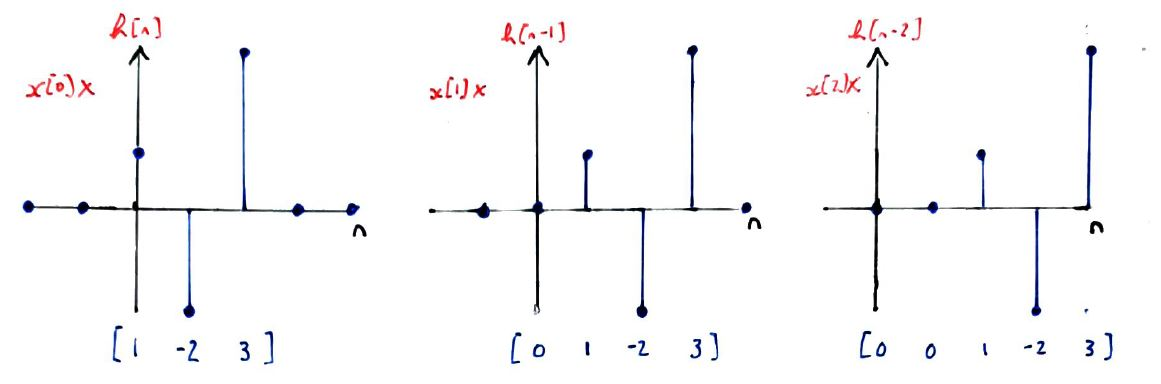
\includegraphics[width=\textwidth]{images/lecture_3_impulse_response_weighting.JPG}
  \caption{
    Each element of the signal $x[k]$ multiplies delayed versions of the impulse
    response $h[n-k]$, resulting in a partial signal. These partial signals are
    then summed to give the convolved signal, $y[n]$.
  }
  \label{fig::lecture_3_impulse_response_weighting}
\end{figure}

\subsection{``Flip and Slide''}
%
Consider the form $h[n-k]$, where $k$ is the dependent variable in our convolutional
sum. Addition of $n$ means the impulse response is first shifted to the left, and
subseqeuntly reflected about the vertical axis (see Figure
\ref{fig::lecture_3_flip_and_slide}).
%
\begin{figure}[!htb]
  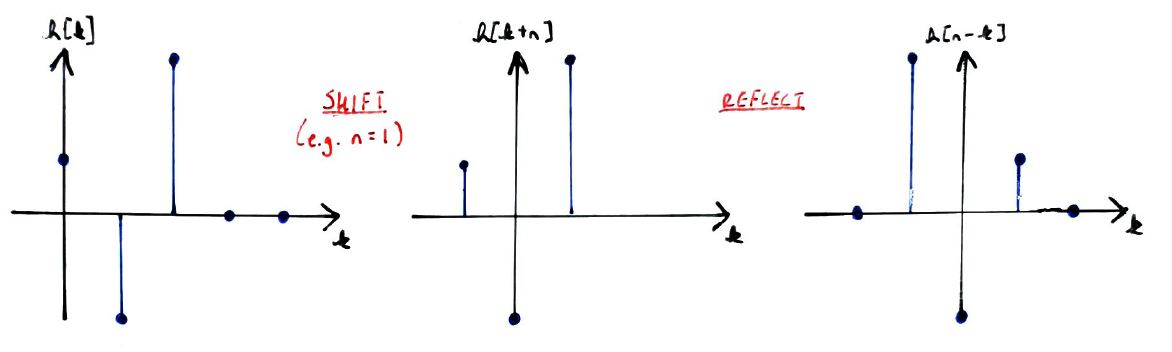
\includegraphics[width=\textwidth]{images/lecture_3_flip_and_slide.JPG}
  \caption{
    Transforming the impulse response so that it can be ``slid'' along the
    signal. Inner products with the signal then yield the convolved signal
    value at a given time.
  }
  \label{fig::lecture_3_flip_and_slide}
\end{figure}
%
The transformed impulse response is then overlapped with the input
signal and an inner product taken, yielding an element of the convolved
signal.

\subsection{Convolutional Array}
%
If it is imperative that one perform a convolution by hand, the simplest
way is probably through the use of an array like that in Figure
\ref{fig::lecture_3_convolution_grid_one}. The rows are enumerated by elements
of the impulse response and the columns by elements of the input signal.
A double line is placed under the element corresponding to the arrays
at $n=0$, and all entries in the matrix are formed by multiplying the
corresponding row and column. Diagonals are then drawn across the array
and elements on the same diagonal are summed to give the result of the
convolution.
%
\begin{figure}[!htb]
  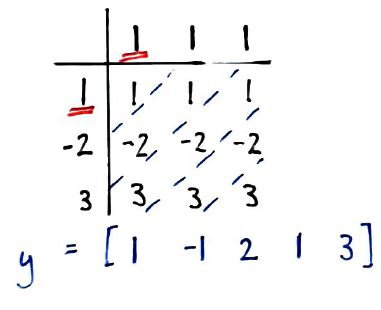
\includegraphics[width=0.3\textwidth]{images/lecture_3_convolution_grid_one.JPG}
  \caption{
    Convolutional array for the signal
    $x = \left[\begin{array}{ccc} 1 & 1 & 1\end{array}\right]$ and
    impulse response
    $h = \left[\begin{array}{ccc} 1 & -2 & 3\end{array}\right]$.
  }
  \label{fig::lecture_3_convolution_grid_one}
\end{figure}
%
In Figure \ref{fig::lecture_3_convolution_grid_one}, we have
$x = \left[\begin{array}{ccc} 1 & 1 & 1\end{array}\right]$ and
$h = \left[\begin{array}{ccc} 1 & -2 & 3\end{array}\right]$. Performing the
summation across diagonals gives the result of the convolution,
$y = \left[\begin{array}{ccccc} 1 & -1 & 2 & 1 & 3\end{array}\right]$. The
zeroth element in $y$ is given by the diagonal containing the multiplication
of underlined elements in the input array, in this case the first diagonal.

\subsection{Properties of LTI Systems}
%
\begin{enumerate}
\item An LTI system is entirely determined by its impulse response. This is \textbf{not} true
  for non-LTI systems. If it's possible to write the response to some special input, e.g. $u[n]$,
  and it is possible to write any other input in terms of this special input, then the response
  to the special input characterises the system
  \footnote{
    Adding a physical analogue for the sake of intuition, consider the problem of characterising
    the acousitics of a room. Ideally, once could produce an instantaneous sound and observe
    the acoustic response, i.e. the signal is $\delta[n]$, and the impulse response is observed.
    However, it's not possible to create a sound like $\delta[n]$ -- some non-zero duration must
    be associated with the noise, and so the input signal is better approximated by $u[n]$. If the
    step response can be characterised, then this can be turned into an impulse response.
  }.\\
  %
\item The convolution is commutative. This can be shown by defining the dummy dependent variable
  $m = n - k$,
  %
  \begin{align*}
    h \circledast x &= \sum_{k=-\infty}^\infty x[k] h[n-k] = \sum_{m=-\infty}^\infty h[m] x[n-m] \\
    &= x \circledast h \,.
  \end{align*}
  %
\item The convolution is distributive:
  %
  \begin{displaymath}
    x \circledast (h_1 + h_2) = x \circledast h_1 + x \circledast h_2 \,.
  \end{displaymath}
  %
\item The convolution is associative:
  %
  \begin{displaymath}
    x \circledast (h_1 \circledast h_2) \Longleftrightarrow (x \circledast h_1) \circledast h_2 \,.
  \end{displaymath}
  %
\item For a causal system, $h[k] = 0$ for $k < 0$. This allows for a simplification in the
  form of the convolution that we've previously used through changing the lower bound of
  the summation:
  %
  \begin{equation}
    y[n] = \sum_{k=0}^\infty h[k]x[n-k] \,.
  \end{equation}
  %
  Were this not the case, $y[n]$ could depend on future values of $x$, and the system would no
  longer be causal.
\end{enumerate}
%
\begin{exmp}
  Let's begin by convolving $x[n] = \alpha^n u[n]$ with $h[n] = u[n]$, where
  $\alpha\in [0,1]$. Given the commutativity of convolution, we can effectively
  choose which function gets ``flipped and slid'' across the other. In this case,
  it will prove easiest to flip and slide the impulse response. In this way, the terms
  in the convolution turn into a geometric progression,
  %
  \begin{displaymath}
    y[-1] = 0, \quad y[0] = 1, \quad y[1] = 1 + \alpha, \quad y[2] = 1 + \alpha + \alpha^2, \hdots
  \end{displaymath}
  %
  \begin{equation}
    y[n] = \left\{\begin{array}{ccl}
    0 & & n < 0 \\
    \sum_{k=0}^n \alpha^k & & \mathrm{otherwise}
    \end{array}\right. = u[n]\sum_{k=0}^n \alpha^k \,.
  \end{equation}
  %
  Recall the elementary identity for the geometric progression when $0\leq\alpha\leq 1$:
  %
  \begin{displaymath}
    \sum_{k=0}^\infty \alpha^k = \frac{1}{1 - \alpha} \,.
  \end{displaymath}
  %
  For the finite sum, we can write this as
  %
  \begin{align*}
    \sum_{k=0}^n \alpha^k &= \sum_{k=0}^\infty \alpha^k - \sum_{k=n+1}^\infty \alpha^k \\
    &= \sum_{k=0}^\infty \alpha^k - \alpha^{n+1}\sum_{k=0}^\infty \alpha^k \\
    &= \frac{1}{1-\alpha} - \frac{\alpha^{n+1}}{1-\alpha} = \frac{1 - \alpha^{n+1}}{1 - \alpha} \,.
  \end{align*}
  %
  It then follows that for our convolution, we have
  %
  \begin{equation}
    y[n] = \frac{1 - \alpha^{n+1}}{1 - \alpha} u[n] \,.
  \end{equation}
  %
  This signal intercepts the vertical axis at $1$ and asymptotes to $\frac{1}{1-\alpha}$.
\end{exmp}
%
\begin{exmp}
  The previous example can actually be treated explicitly:
  %
  \begin{align*}
    y[n] &= \sum_{k=-\infty}^\infty x[k]h[n-k] = \sum_{k=-\infty}^\infty \alpha^k u[k] u[n-k] \\
    &= \sum_{k=0}^\infty \alpha^k u[n-k] = \sum_{k=0}^\infty \alpha^k \,,
  \end{align*}
  %
  where the second line omits the summation from $-\infty$ to $-1$ since $u[k] = 0$ for $k < 0$.
\end{exmp}
